\chapter{pH और चालकता द्वारा अनुमापन}\label{ch:g12:ph-conductivity-titrations}

वाइन सिरके की एक बोतल पर लिखा है ``6 \% अम्लता'': सिरके के हर सौ ग्राम में
एथेनोइक अम्ल के छह ग्राम। न एथेनोइक अम्ल रंगीन है, न
उसका संयुग्मी क्षारक, और यहाँ कोई परमैंगनेट मदद नहीं करेगा।
पर सिरके में डुबोया गया \omterm{def:g9:acids-bases-ph:ph-paper}{pH मीटर}, या यह मापने वाला सेल कि वह कितनी अच्छी तरह
चालन करता है, किसी क्षारक के साथ अभिक्रिया का बूँद-बूँद पीछा करता है, और वक्र की
आकृति ठीक-ठीक दिखा देती है कि \omterm{def:g11:titration:equivalence}{तुल्यता} कहाँ है। मेज़ पर दस मिनट,
और लेबल की जाँच हो जाती है।

\begin{recall}
\omterm{def:g11:titration:titration}{अनुमापन}, उसकी \omterm{def:g11:titration:equivalence}{तुल्यता} और \omterm{def:g11:titration:equivalence}{तुल्यता आयतन}
(\cref{ch:g11:titration}); \omterm{def:g12:ka-and-pka:ka}{अम्लता स्थिरांक} (\cref{ch:g12:ka-and-pka});
हेंडरसन संबंध और सूचक
(\cref{ch:g12:buffers-predominance}); \omterm{def:g9:ions:ion}{आयनों} के विलयन विद्युत का
चालन करते हैं (\cref{ch:g9:ions})।
\end{recall}

\begin{omfigure}
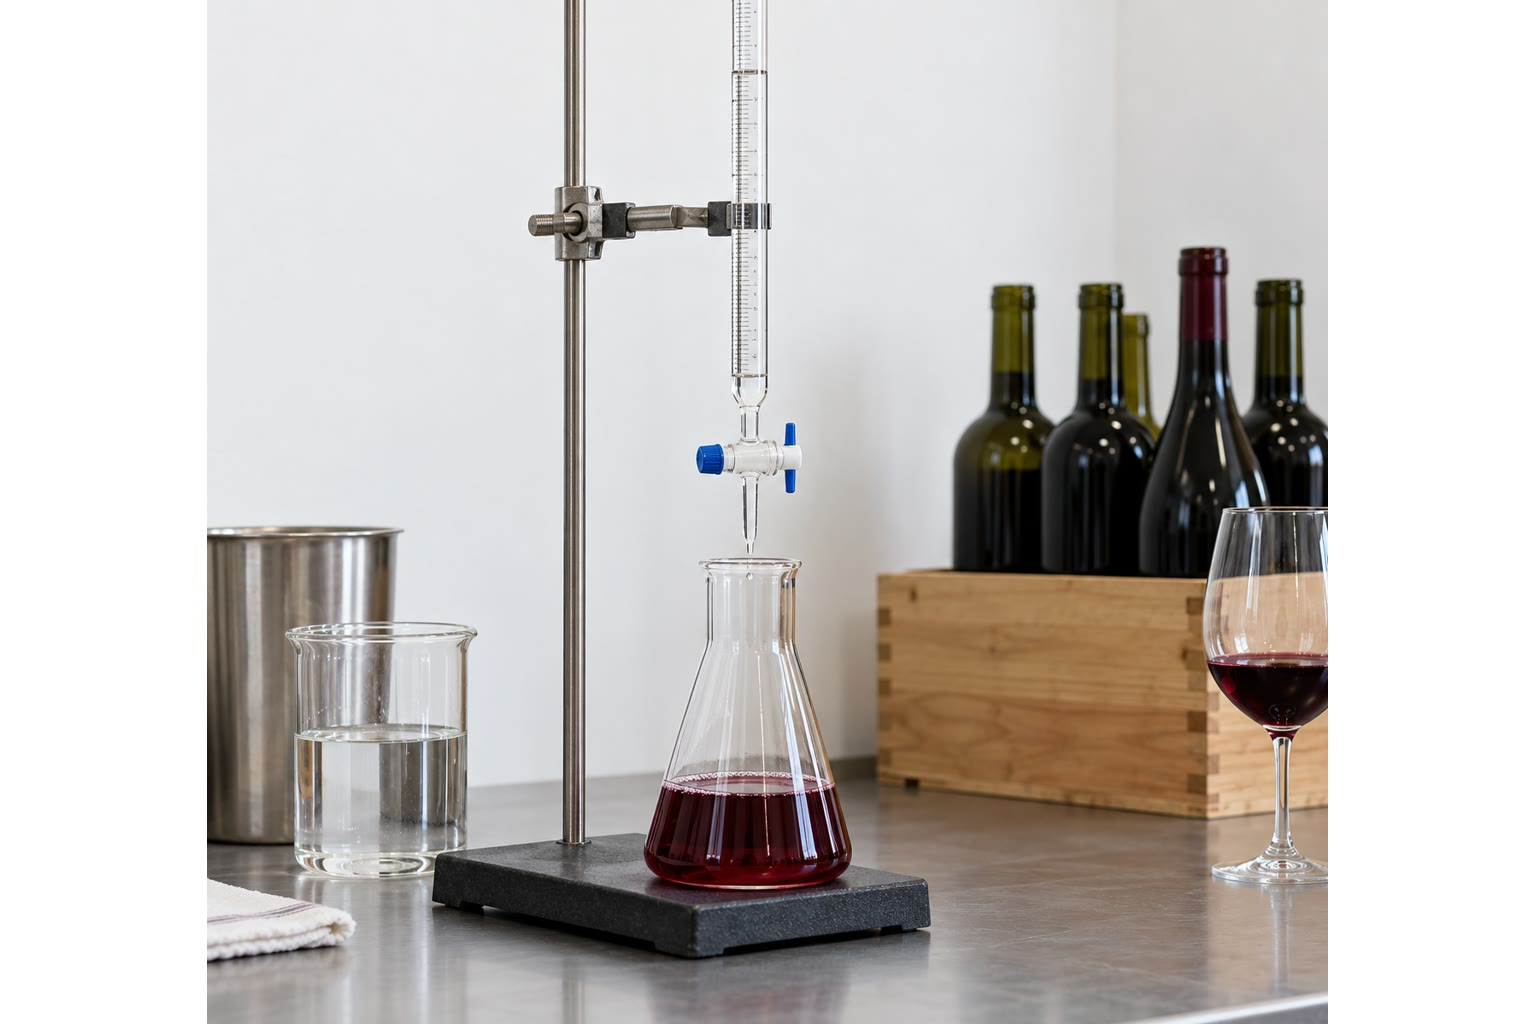
\includegraphics[width=0.45\linewidth]{images/book1/ai/g12-wine-lab.jpg}

{\small वाइन बनाने वाले की \omterm{def:g11:titration:titration}{अनुमापन} मेज़।}
\end{omfigure}

\section{pH-मितीय अनुमापन}

\begin{definition}[pH-मितीय अनुमापन, अर्ध-तुल्यता]\label{def:g12:ph-conductivity-titrations:ph-metric}
\emph{pH-मितीय अनुमापन}\index{pH-मितीय अनुमापन} में \omterm{def:g11:titration:titration}{अनुमापक} के हर बार मिलाने के बाद
\omterm{def:g11:titration:titration}{अनुमापित विलयन} का \omterm{def:g9:acids-bases-ph:ph}{pH} मापा जाता है, और मिलाए गए आयतन के विरुद्ध
\omterm{def:g9:acids-bases-ph:ph}{pH} का वक्र बनाया जाता है। \emph{अर्ध-तुल्यता}\index{अर्ध-तुल्यता}
वह बिंदु है जहाँ \omterm{def:g11:titration:equivalence}{तुल्यता आयतन} का आधा मिलाया जा चुका हो।
\end{definition}

\begin{omfigure}
\begin{tikzpicture}[font=\small, scale=0.65]
  \pic[transform shape] at (0,0) {stand={6.3}{2.0}};
  \pic[transform shape] at (2.0,0.68) {stirrer};
  \pic[transform shape] at (2.0,0.68) {beaker={0.45}{omWater}};
  \pic[transform shape] at (2.0,2.9) {burette={0.8}{omWater}};
  \pic[transform shape] (pr) at (2.6,0.95) {probe};
  \pic[transform shape] (m) at (6.4,3.4) {meter={pH}};
  \draw[black!70, thick] (pr-top) .. controls +(0,1.0) and +(0,-1.2) .. (m-a);
  \draw[omProp, thick, <-] (2.35,7.2) -- (4.3,7.6) node[right, text=black] {ब्यूरेट: NaOH};
  \draw[omProp, thick, <-] (1.4,1.1) -- (-1.4,1.6) node[left, text=black, align=right] {अनुमापित किया जाने वाला अम्ल};
  \draw[omProp, thick, <-] (2.75,2.4) -- (4.3,2.0) node[right, text=black] {pH प्रोब};
\end{tikzpicture}

{\small एक \omterm{def:g12:ph-conductivity-titrations:ph-metric}{pH-मितीय अनुमापन}: प्रोब विलोडित विलयन में डूबा है,
मीटर हर बार मिलाने के बाद \omterm{def:g9:acids-bases-ph:ph}{pH} दिखाता है।}
\end{omfigure}

\begin{inthelab}[pH मीटर का अंशांकन]
उपयोग से पहले प्रोब को आसुत जल से खँगालकर ज्ञात \omterm{def:g9:acids-bases-ph:ph}{pH} वाले दो
\omterm{def:g12:buffers-predominance:buffer}{बफ़र विलयनों} में डुबोया जाता है, आम तौर पर 7.0 और 4.0 (या 10.0): मीटर
को उनके मान पढ़ने के लिए समायोजित किया जाता है। दो विलयनों के बीच प्रोब को खँगालकर
धीरे से थपथपाकर सुखाया जाता है, कभी रगड़ा नहीं जाता; उसे गीली नोक के साथ रखा जाता है।
\end{inthelab}

\begin{omfigure}
\begin{minipage}{0.49\linewidth}
\begin{tikzpicture}
\begin{axis}[width=\linewidth, height=6cm, xmin=0, xmax=30, ymin=0, ymax=14,
    xlabel={$V_{\text{NaOH}}$ (\si{mL})}, ylabel={pH}, axis lines*=left,
    ymajorgrids, grid style={gray!20}, tick label style={font=\scriptsize},
    label style={font=\small}, title={\small \ce{HCl} का \ce{NaOH} से अनुमापन},
    title style={yshift=-4pt}]
  \addplot[very thick, omDef] table[x=V, y=pH] {figdata/out/grade-12-ph-conductivity-titrations-a.dat};
  \addplot[thick, omProp, densely dotted] table[x=V, y expr=\thisrow{dpH}/4]
    {figdata/out/grade-12-ph-conductivity-titrations-a.dat};
  \addplot[dashed, black!60] coordinates {(20,0) (20,7)};
  \node[font=\scriptsize, anchor=north west] at (axis cs:20.3,6.5) {$V_E = 20.0$};
\end{axis}
\end{tikzpicture}
\end{minipage}\hfill
\begin{minipage}{0.49\linewidth}
\begin{tikzpicture}
\begin{axis}[width=\linewidth, height=6cm, xmin=0, xmax=16, ymin=0, ymax=14,
    xlabel={$V_{\text{NaOH}}$ (\si{mL})}, ylabel={pH}, axis lines*=left,
    ymajorgrids, grid style={gray!20}, tick label style={font=\scriptsize},
    label style={font=\small}, title={\small \ce{CH3COOH} का \ce{NaOH} से अनुमापन},
    title style={yshift=-4pt}]
  \addplot[very thick, omDef] table[x=V, y=pH] {figdata/out/grade-12-ph-conductivity-titrations-b.dat};
  \addplot[thick, omProp, densely dotted] table[x=V, y expr=\thisrow{dpH}/4]
    {figdata/out/grade-12-ph-conductivity-titrations-b.dat};
  \addplot[dashed, black!60] coordinates {(10.1,0) (10.1,8.7)};
  \addplot[dashed, black!60] coordinates {(0,4.76) (5.05,4.76) (5.05,0)};
  \node[font=\scriptsize, anchor=south west] at (axis cs:0.2,4.8) {$pK_a = 4.76$};
  \node[font=\scriptsize, anchor=north west] at (axis cs:10.4,3.0) {$V_E = 10.1$};
\end{axis}
\end{tikzpicture}
\end{minipage}

{\small परिकलित \omterm{def:g9:acids-bases-ph:ph}{pH} वक्र (नीले) और उनका अवकलज $d\mathrm{pH}/dV$
(नारंगी, बिंदुदार, 4 से विभाजित)। बाएँ: \qty{0.100}{mol/L} हाइड्रोक्लोरिक अम्ल
के \qty{20.0}{mL}; \omterm{def:g11:titration:equivalence}{तुल्यता} \omterm{def:g9:acids-bases-ph:ph}{pH} 7.00 पर। दाएँ: तनु सिरके के \qty{10.0}{mL};
\omterm{def:g12:ph-conductivity-titrations:ph-metric}{अर्ध-तुल्यता} पर \omterm{def:g9:acids-bases-ph:ph}{pH}, $pK_a$ के बराबर होता है, और
\omterm{def:g11:titration:equivalence}{तुल्यता} क्षारकीय \omterm{def:g9:acids-bases-ph:ph}{pH} पर होती है।}
\end{omfigure}


\begin{method}[अवकलज विधि]\label{met:g12:ph-conductivity-titrations:derivative}
क्रमागत मापों के बीच प्रवणता
$\Delta\mathrm{pH}/\Delta V$ निकालिए, और उसे $V$ के विरुद्ध आलेखित कीजिए (स्प्रेडशीट या
कैलकुलेटर यह कर देता है)। \omterm{def:g11:titration:equivalence}{तुल्यता आयतन} वहाँ है जहाँ यह प्रवणता
सबसे बड़ी हो: अवकलज वक्र का शिखर।
\end{method}

\begin{method}[स्पर्शरेखा विधि]\label{met:g12:ph-conductivity-titrations:tangent}
\begin{enumerate}
  \item वक्र पर दो समांतर स्पर्शरेखाएँ खींचिए, एक उछाल से पहले और एक उसके
        बाद, उसके दोनों ओर।
  \item उनके ठीक बीच में समांतर रेखा खींचिए।
  \item जहाँ वह वक्र को काटती है, वही \omterm{def:g11:titration:equivalence}{तुल्यता} बिंदु है: $V_E$ (और
        \omterm{def:g11:titration:equivalence}{तुल्यता} पर \omterm{def:g9:acids-bases-ph:ph}{pH}) पढ़िए।
\end{enumerate}
\end{method}

\begin{proposition}[अर्ध-तुल्यता पर $\mathrm{pH} = pK_a$]\label{prop:g12:ph-conductivity-titrations:half}
किसी \omterm{def:g12:ka-and-pka:strong-acid}{प्रबल क्षारक} द्वारा \omterm{def:g12:ka-and-pka:strong-acid}{दुर्बल अम्ल} \ce{HA} के \omterm{def:g11:titration:titration}{अनुमापन} में
\omterm{def:g12:ph-conductivity-titrations:ph-metric}{अर्ध-तुल्यता} पर $\mathrm{pH} = pK_a$।
\end{proposition}

\begin{proof}
अभिक्रिया \ce{HA + OH- -> A- + H2O} पूर्ण है। \omterm{def:g12:ph-conductivity-titrations:ph-metric}{अर्ध-तुल्यता} पर
आधा अम्ल \ce{A-} में बदल चुका होता है: $[\ce{A-}] = [\ce{HA}]$, और
हेंडरसन संबंध $\mathrm{pH} = pK_a + \log 1 = pK_a$ देता है।
\end{proof}

\begin{remark}[वक्र से सूचक चुनना]\label{rem:g12:ph-conductivity-titrations:indicator}
% ledger: ind:BBT, ind:phenolphthalein
सूचक को उछाल के भीतर रंग बदलना चाहिए। हाइड्रोक्लोरिक अम्ल के लिए
उछाल लगभग \omterm{def:g9:acids-bases-ph:ph}{pH} 4 से 10 तक फैला होता है और कई सूचक उपयुक्त हैं, ब्रोमोथाइमॉल ब्लू
सबसे अच्छा; एथेनोइक अम्ल के लिए उछाल छोटा और क्षारकीय होता है, लगभग 7 से 11:
फ़ीनॉल्फ़्थेलीन (8.0--10.0) उपयुक्त है, ब्रोमोथाइमॉल ब्लू बहुत
जल्दी बदल जाता।
\end{remark}

\section{चालकता और चालकतामितीय अनुमापन}

\begin{definition}[चालकता, मोलर आयनिक चालकता]\label{def:g12:ph-conductivity-titrations:conductivity}
किसी विलयन की \emph{चालकता}\index{चालकता} $\sigma$
मापती है कि वह विद्युत का कितना अच्छा चालन करता है; इसे चालकतामापी पर
\si{mS/cm} (या \si{S/m}) में पढ़ा जाता है। हर \omterm{def:g9:ions:ion}{आयन} $i$ अपनी सांद्रता के
अनुपात में, एक गुणांक $\lambda_i$ के साथ, इसमें योगदान देता है, जो उसकी
\emph{मोलर आयनिक चालकता}\index{मोलर आयनिक चालकता} है।
\end{definition}

\begin{proposition}[कोलराउश नियम]\label{prop:g12:ph-conductivity-titrations:kohlrausch}
% ledger: lam:H+, lam:OH-, lam:Na+, lam:Cl-
तनु विलयन के लिए $\sigma = \sum_i \lambda_i [X_i]$।
\qty{25}{\celsius} पर, \si{S.cm^2/mol} में: \ce{H3O+} 349.8, \ce{OH-} 198.3,
\ce{Cl-} 76.2, \ce{Na+} 50.3। ऑक्सोनियम और हाइड्रॉक्साइड \omterm{def:g9:ions:ion}{आयन} अन्य सभी \omterm{def:g9:ions:ion}{आयनों} से
कहीं बेहतर चालन करते हैं।
\end{proposition}

\begin{proof}
स्वीकृत (विश्वविद्यालय के प्रथम वर्ष का खंड)। \ce{Cl-} और \ce{Na+} के मान
हाइड्रोक्लोरिक अम्ल और सोडियम क्लोराइड विलयनों की मापी गई \omterm{def:g12:ph-conductivity-titrations:conductivity}{चालकताओं} से आते हैं,
जिनमें से \ce{H3O+} की \omterm{def:g12:ph-conductivity-titrations:conductivity}{चालकता} घटा दी जाती है।
\end{proof}

\begin{definition}[चालकतामितीय अनुमापन]\label{def:g12:ph-conductivity-titrations:conductimetric}
\emph{चालकतामितीय अनुमापन}\index{चालकतामितीय अनुमापन} में
\omterm{def:g11:titration:titration}{अनुमापक} के हर बार मिलाने के बाद \omterm{def:g12:ph-conductivity-titrations:conductivity}{चालकता} मापी जाती है। \omterm{def:g11:titration:titration}{अनुमापित
विलयन} को पानी के बड़े आयतन में तनु किया जाता है, ताकि मिलाया गया
आयतन उसे मुश्किल से बदले: तब बिंदु सीधी रेखाओं पर होते हैं, जो
\omterm{def:g11:titration:equivalence}{तुल्यता} पर अपनी प्रवणता बदलती हैं।
\end{definition}

\begin{omfigure}
\begin{minipage}{0.4\linewidth}\centering
\begin{tikzpicture}[font=\small, scale=0.75]
  \pic[transform shape] at (0,0) {beaker={0.6}{omWater}};
  \pic[transform shape] (cc) at (0.2,0.2) {condcell};
  \pic[transform shape] (m) at (2.6,3.4) {meter={mS/cm}};
  \draw[black!70, thick] (cc-top) .. controls +(0,0.8) and +(0,-1) .. (m-a);
  \node[anchor=north, align=center] at (0.6,-0.15) {विलयन में\\ चालकतामापी सेल};
\end{tikzpicture}
\end{minipage}\hfill
\begin{minipage}{0.56\linewidth}
\begin{tikzpicture}
\begin{axis}[width=\linewidth, height=5.4cm, xmin=0, xmax=20, ymin=0,
    ymax=4.6, xlabel={$V_{\text{NaOH}}$ (\si{mL})}, ylabel={$\sigma$ (\si{mS/cm})},
    axis lines*=left, ymajorgrids, grid style={gray!20},
    tick label style={font=\scriptsize}, label style={font=\small}]
  \addplot[only marks, mark=*, mark size=1.4pt, omDef] table[x=V, y=sigma]
    {figdata/out/grade-12-ph-conductivity-titrations-c.dat};
  \addplot[dashed, black!60] coordinates {(10,0) (10,4.6)};
  \node[font=\scriptsize, anchor=south west] at (axis cs:10.3,0.2) {$V_E = 10.0$};
\end{axis}
\end{tikzpicture}
\end{minipage}

{\small बाएँ: एक चालकतामापी सेल। दाएँ: \qty{0.0100}{mol/L} हाइड्रोक्लोरिक
अम्ल के \qty{100}{mL} का
\qty{0.100}{mol/L} सोडियम हाइड्रॉक्साइड से \omterm{def:g11:titration:titration}{अनुमापन} (कोलराउश नियम से परिकलित)। \omterm{def:g12:ph-conductivity-titrations:conductivity}{चालकता}
घटती है, फिर बढ़ती है: \omterm{def:g11:titration:equivalence}{तुल्यता} पर मिलने वाली दो सीधी रेखाएँ।}
\end{omfigure}

\begin{example}[दोनों रेखाएँ पढ़ना]\label{ex:g12:ph-conductivity-titrations:lines}
\omterm{def:g11:titration:equivalence}{तुल्यता} से पहले मिलाया गया हर \ce{OH-} एक \ce{H3O+}
($\lambda = 349.8$) हटाता है और एक \ce{Na+} ($\lambda = 50.3$) लाता है:
\omterm{def:g12:ph-conductivity-titrations:conductivity}{चालकता} तेज़ी से घटती है। \omterm{def:g11:titration:equivalence}{तुल्यता} के बाद \ce{Na+} और \ce{OH-}
($\lambda = 198.3$) बस जमा होते जाते हैं: वह बढ़ती है। दोनों रेखाएँ
$V_E = \qty{10.0}{mL}$ पर मिलती हैं, इसलिए अम्ल
$0.100 \times 10.0 / 100 = \qty{0.0100}{mol/L}$ था।
\end{example}

\begin{method}[चालकतामितीय अनुमापन से तुल्यता]\label{met:g12:ph-conductivity-titrations:two-lines}
\omterm{def:g11:titration:equivalence}{तुल्यता} से पहले के बिंदुओं से होकर सबसे उपयुक्त सीधी रेखा खींचिए, और
उसके बाद के बिंदुओं से होकर सबसे उपयुक्त रेखा; $V_E$ उनके
प्रतिच्छेदन पर पढ़िए। \omterm{def:g11:titration:equivalence}{तुल्यता} के निकट के बिंदु, जहाँ रेखाएँ मुड़ती हैं, छोड़ दिए
जाते हैं।
\end{method}

\begin{remark}[कौन-सी विधि कब]\label{rem:g12:ph-conductivity-titrations:which}
जब कोई उपयुक्त रंगीन सूचक उपलब्ध हो, तो वही सबसे तेज़ है। \omterm{def:g12:ph-conductivity-titrations:ph-metric}{pH-मितीय
अनुमापन} \omterm{def:g12:ka-and-pka:strong-acid}{दुर्बल अम्ल} का $pK_a$ भी देता है, और रंगीन
या धुँधले विलयनों के साथ भी काम करता है। \omterm{def:g12:ph-conductivity-titrations:conductimetric}{चालकतामितीय अनुमापन} को \omterm{def:g9:acids-bases-ph:ph}{pH} में किसी उछाल की
ज़रूरत ही नहीं: यह बहुत दुर्बल या बहुत तनु अम्लों के लिए, और \omterm{def:g9:ions:precipitate}{अवक्षेपण}
अभिक्रियाओं के लिए भी काम करता है, जब तक \omterm{def:g9:ions:ion}{आयन} बदलते हैं।
\end{remark}

\begin{safety}{\ghs[0.82cm]{GHS05}\ghs[0.82cm]{GHS07}}
% ledger: ghs:NaOH
सोडियम हाइड्रॉक्साइड विलयन त्वचा और आँखों को जलाते हैं, आँखों में तो तनु विलयन
भी: पूरे समय चश्मा, और कोई भी छींटा तुरंत
भरपूर पानी से धोया जाए।
\end{safety}

\section{अभ्यास}


\begin{exercise}[$\star$]\label{exo:g12:ph-conductivity-titrations:1}
\qty{0.100}{mol/L} सोडियम हाइड्रॉक्साइड द्वारा अनुमापित हाइड्रोक्लोरिक अम्ल के
वक्र पर \omterm{def:g11:titration:equivalence}{तुल्यता आयतन} पढ़िए, और अम्ल के
\qty{20.0}{mL} की सांद्रता निकालिए।
\end{exercise}

\begin{exercise}[$\star$]\label{exo:g12:ph-conductivity-titrations:2}
एक \omterm{def:g12:ka-and-pka:strong-acid}{दुर्बल अम्ल} का सोडियम हाइड्रॉक्साइड से \omterm{def:g11:titration:titration}{अनुमापन} किया जाता है; $V_E = \qty{12.0}{mL}$।
\qty{6.0}{mL} पर \omterm{def:g9:acids-bases-ph:ph}{pH} 3.75 है। अम्ल का $pK_a$ बताइए। $pK_a$ पैमाने का
कौन-सा अम्ल यह हो सकता है?
\end{exercise}

\begin{exercise}[$\star$]\label{exo:g12:ph-conductivity-titrations:3}
सोडियम हाइड्रॉक्साइड द्वारा एथेनोइक अम्ल के \omterm{def:g11:titration:titration}{अनुमापन} के लिए आप कौन-सा सूचक
चुनेंगे? मेथिल रेड क्यों नहीं?
\end{exercise}

\begin{exercise}[$\star$]\label{exo:g12:ph-conductivity-titrations:4}
\omterm{def:g9:acids-bases-ph:ph-paper}{pH मीटर} का उपयोग से पहले अंशांकन क्यों आवश्यक है? किससे?
\end{exercise}

\begin{exercise}[$\star$]\label{exo:g12:ph-conductivity-titrations:5}
\omterm{def:g12:ph-conductivity-titrations:conductivity}{मोलर आयनिक चालकताओं} की मदद से \omterm{def:g9:ions:ion}{आयनों} \ce{H3O+}, \ce{OH-},
\ce{Na+}, \ce{Cl-} को सबसे अच्छे चालक से सबसे ख़राब के क्रम में रखिए।
\end{exercise}

\begin{exercise}[$\star\star$]\label{exo:g12:ph-conductivity-titrations:6}
एथेनोइक अम्ल विलयन के \qty{20.0}{mL} को \qty{0.050}{mol/L} सोडियम हाइड्रॉक्साइड के
\qty{14.6}{mL} की आवश्यकता होती है। उसकी सांद्रता निकालिए।
\end{exercise}

\begin{exercise}[$\star\star$]\label{exo:g12:ph-conductivity-titrations:7}
\omterm{def:g11:titration:equivalence}{तुल्यता} के निकट पाठ्यांक हैं: \qty{9.6}{mL}, \omterm{def:g9:acids-bases-ph:ph}{pH} 5.7;
\qty{9.8}{mL}, 6.1; \qty{10.0}{mL}, 7.0; \qty{10.2}{mL}, 10.5;
\qty{10.4}{mL}, 11.0। क्रमागत बिंदुओं के बीच $\Delta\mathrm{pH}/\Delta V$
निकालिए और $V_E$ ज्ञात कीजिए।
\end{exercise}

\begin{exercise}[$\star\star$]\label{exo:g12:ph-conductivity-titrations:8}
हाइड्रोक्लोरिक अम्ल के \omterm{def:g12:ph-conductivity-titrations:conductimetric}{चालकतामितीय अनुमापन} में, मौजूद \omterm{def:g9:ions:ion}{आयनों} की मदद से, \omterm{def:g11:titration:equivalence}{तुल्यता} से पहले और
उसके बाद प्रवणता के चिह्न को समझाइए।
\end{exercise}

\begin{exercise}[$\star\star$]\label{exo:g12:ph-conductivity-titrations:9}
सोडियम हाइड्रॉक्साइड द्वारा अनुमापित एथेनोइक अम्ल का चालकतामितीय वक्र रेखांकित कीजिए।
\omterm{def:g11:titration:equivalence}{तुल्यता} से पहले भी \omterm{def:g12:ph-conductivity-titrations:conductivity}{चालकता} क्यों बढ़ती है?
\end{exercise}

\begin{exercise}[$\star\star$]\label{exo:g12:ph-conductivity-titrations:10}
तनु सिरके के परिकलित वक्र पर आरंभ में,
\omterm{def:g12:ph-conductivity-titrations:ph-metric}{अर्ध-तुल्यता} पर और \omterm{def:g11:titration:equivalence}{तुल्यता} पर \omterm{def:g9:acids-bases-ph:ph}{pH} पढ़िए। आरंभिक \omterm{def:g9:acids-bases-ph:ph}{pH} उसी सांद्रता के
हाइड्रोक्लोरिक अम्ल के \omterm{def:g9:acids-bases-ph:ph}{pH} से कहीं अधिक क्यों है?
\end{exercise}

\begin{exercise}[$\star\star$]\label{exo:g12:ph-conductivity-titrations:11}
\omterm{def:g12:ph-conductivity-titrations:conductimetric}{चालकतामितीय अनुमापन} से पहले \omterm{def:g11:titration:titration}{अनुमापित विलयन} को पानी के बड़े आयतन में
क्यों तनु किया जाता है?
\end{exercise}

\begin{exercise}[$\star\star\star$]\label{exo:g12:ph-conductivity-titrations:12}
एक विलयन में हाइड्रोक्लोरिक अम्ल और एथेनोइक अम्ल दोनों हैं। \omterm{def:g9:acids-bases-ph:ph}{pH} मापते हुए
सोडियम हाइड्रॉक्साइड से उसका \omterm{def:g11:titration:titration}{अनुमापन} किया जाता है। समझाइए कि
वक्र में दो उछाल क्यों दिखते हैं, और हर \omterm{def:g11:titration:equivalence}{तुल्यता आयतन} क्या मापता है।
\end{exercise}

\begin{exercise}[$\star\star\star$]\label{exo:g12:ph-conductivity-titrations:13}
अध्याय के \omterm{def:g12:ph-conductivity-titrations:conductimetric}{चालकतामितीय अनुमापन} के आरंभ में (\qty{0.0100}{mol/L} हाइड्रोक्लोरिक अम्ल)
और \omterm{def:g11:titration:equivalence}{तुल्यता} पर (सोडियम क्लोराइड विलयन के \qty{110}{mL}) \omterm{def:g12:ph-conductivity-titrations:conductivity}{चालकता}
निकालिए। चित्र से तुलना कीजिए।
\end{exercise}

\begin{exercise}[$\star\star\star$]\label{exo:g12:ph-conductivity-titrations:14}
ग़लत अंशांकित एक \omterm{def:g9:acids-bases-ph:ph-paper}{pH मीटर} हर \omterm{def:g9:acids-bases-ph:ph}{pH} को 0.2 अधिक पढ़ता है। इससे \omterm{def:g12:ph-conductivity-titrations:ph-metric}{pH-मितीय अनुमापन} के
\omterm{def:g11:titration:equivalence}{तुल्यता आयतन} पर कौन-सी त्रुटि आती है? \omterm{def:g12:ph-conductivity-titrations:ph-metric}{अर्ध-तुल्यता} पर पढ़े गए $pK_a$
पर?
\end{exercise}

\begin{exercise}[$\star\star\star$]\label{exo:g12:ph-conductivity-titrations:15}
\omterm{def:g12:ph-conductivity-titrations:conductimetric}{चालकतामितीय अनुमापन} सिल्वर \omterm{def:g9:ions:ion}{आयनों} की क्लोराइड \omterm{def:g9:ions:ion}{आयनों} के साथ अभिक्रिया,
\ce{Ag+ + Cl- -> AgCl(s)}, का पीछा क्यों कर सकता है, जबकि \omterm{def:g12:ph-conductivity-titrations:ph-metric}{pH-मितीय
अनुमापन} नहीं कर सकता? सोडियम क्लोराइड में सिल्वर नाइट्रेट मिलाने पर अपेक्षित
वक्र का वर्णन कीजिए (\ce{NO3-} का $\lambda$ \ce{Cl-} वाले मान के
निकट मानिए)।
\end{exercise}

\section{समस्या: क्या सिरका 6\,\% है?}

\begin{problem}[{सप्ताहांत समस्या --- क्या ``6 \% अम्लता'' अंकित सिरके में
वास्तव में प्रति सौ ग्राम छह ग्राम एथेनोइक अम्ल है?}]
\label{pb:g12:ph-conductivity-titrations:1}
% ledger: pka:ethanoic, ind:phenolphthalein, lam:OH-, lam:Na+, aw:C, aw:H, aw:O
``6 \% अम्लता'' अंकित एक सिरके की जाँच की जाती है। उसके \qty{100.0}{mL}
तौले जाते हैं: \qty{101}{g}। सिरके को दस गुना तनु किया जाता है, फिर
तनु विलयन के \qty{10.0}{mL} का \qty{0.100}{mol/L} सोडियम हाइड्रॉक्साइड से
\omterm{def:g9:acids-bases-ph:ph-paper}{pH मीटर} के साथ \omterm{def:g11:titration:titration}{अनुमापन} किया जाता है; अध्याय का परिकलित वक्र
(दाएँ) मापों से मेल खाता है।

\medskip
\noindent\textbf{भाग I --- नमूना तैयार करना।}
\begin{enumerate}
  \item ``6 \% अम्लता'' का क्या अर्थ है?
  \item यदि लेबल सही है, तो सिरके के \qty{100.0}{mL} में एथेनोइक अम्ल का कितना
        द्रव्यमान है? यह कौन-सी \omterm{def:g10:concentration-and-dilution:molar-concentration}{मोलर सांद्रता}
        है?
  \item \omterm{def:g11:titration:titration}{अनुमापन} से पहले सिरके को तनु क्यों किया जाता है?
  \item उसे दस गुना तनु करने के लिए काँच के कौन-से उपकरण इस्तेमाल होते हैं?
\end{enumerate}

\medskip
\noindent\textbf{भाग II --- \omterm{def:g12:ph-conductivity-titrations:ph-metric}{pH-मितीय अनुमापन}।}
\begin{enumerate}[resume]
  \item \omterm{def:g11:titration:titration}{अनुमापन} अभिक्रिया का समीकरण लिखिए।
  \item वक्र पर \omterm{def:g11:titration:equivalence}{तुल्यता आयतन} पढ़िए।
  \item तनु सिरके की सांद्रता निकालिए।
  \item उससे सिरके की सांद्रता निकालिए।
  \item \omterm{def:g12:ph-conductivity-titrations:ph-metric}{अर्ध-तुल्यता} पर \omterm{def:g9:acids-bases-ph:ph}{pH} पढ़िए। इससे क्या मिलता है?
  \item \omterm{def:g11:titration:equivalence}{तुल्यता} पर \omterm{def:g9:acids-bases-ph:ph}{pH} 7 से ऊपर क्यों है?
  \item कौन-सा सूचक यही परिणाम देता?
\end{enumerate}

\medskip
\noindent\textbf{भाग III --- चालकतामितीय जाँच।}
\begin{enumerate}[resume]
  \item \omterm{def:g11:titration:titration}{अनुमापन} को चालकतामापी सेल के साथ दोहराया जाता है, नमूने को
        \qty{200}{mL} पानी में तनु करके। \omterm{def:g11:titration:equivalence}{तुल्यता} से पहले विलयन में कौन-से \omterm{def:g9:ions:ion}{आयन}
        प्रकट होते हैं?
  \item \omterm{def:g11:titration:equivalence}{तुल्यता} से पहले \omterm{def:g12:ph-conductivity-titrations:conductivity}{चालकता} केवल धीरे-धीरे क्यों बढ़ती है?
  \item उसके बाद वह तेज़ी से क्यों बढ़ती है?
  \item आरंभ में \omterm{def:g12:ph-conductivity-titrations:conductivity}{चालकता} बहुत कम क्यों होती है?
  \item दोनों रेखाएँ कहाँ मिलनी चाहिए?
\end{enumerate}

\medskip
\noindent\textbf{भाग IV --- निर्णय।}
\begin{enumerate}[resume]
  \item सिरके में एथेनोइक अम्ल की \omterm{def:g10:concentration-and-dilution:mass-concentration}{द्रव्यमान सांद्रता} निकालिए।
  \item सिरके के \qty{100.0}{mL} में एथेनोइक अम्ल का द्रव्यमान निकालिए।
  \item सिरके के प्रति \qty{100}{g} एथेनोइक अम्ल का द्रव्यमान निकालिए।
  \item अंतिम उत्तर बताइए: सिरके की अम्लता क्या है?
\end{enumerate}
\end{problem}
